% ======================================================================
%  AxiSim Software Manual  v1.05-alpha
%  ---------------------------------------------------------------------
%  Drop-in Overleaf project. All diagrams are native TikZ. Screenshots
%  are optional: to enable them in Overleaf, create an "images/" folder
%  and upload the following files. In the repository they already exist
%  under docs/images/ with these names:
%
%     images/ui_sketch.png        (Geometry tab, ribbon + grid)
%     images/ui_mesh.png          (Mesh tab, structured mesh + statistics)
%     images/ui_solver.png        (Solver tab, solver settings + residuals)
%     images/ui_transient.png     (Solver tab, transient settings)
%     images/ui_results.png       (Results tab, 3D view + 2D inspector)
%     images/ui_mirror.png        (Results tab, mirrored inspector)
%
%  If you do NOT want screenshots yet, set \showscreenshotsfalse below
%  and the figures become captioned placeholders so the document still
%  compiles cleanly.
% ======================================================================
\documentclass[11pt]{article}

\usepackage[margin=1in]{geometry}
\usepackage[T1]{fontenc}
\usepackage{lmodern}
\usepackage{amsmath,amssymb}
\usepackage{graphicx}
\usepackage{booktabs}
\usepackage{array}
\usepackage{xcolor}
\usepackage{subcaption}
\usepackage{enumitem}
\usepackage{listings}
\usepackage{tikz}
\usetikzlibrary{arrows.meta,positioning,calc,shapes.geometric}
\usepackage[hidelinks]{hyperref}

\graphicspath{{images/}}

% ---- toggle screenshots on/off ----
\newif\ifshowscreenshots
\showscreenshotstrue   % <- set to \showscreenshotsfalse to use placeholders

% helper: include a screenshot if enabled, else a placeholder box
\newcommand{\screenshot}[3]{% {file}{width}{placeholder caption}
  \ifshowscreenshots
    \includegraphics[width=#2]{#1}%
  \else
    \fbox{\parbox[c][0.42\textwidth][c]{#2}{\centering\itshape screenshot placeholder:\\ #3}}%
  \fi
}

% ---- listings style for code / console ----
\definecolor{codebg}{RGB}{246,247,249}
\definecolor{codekw}{RGB}{0,90,160}
\definecolor{codecm}{RGB}{110,120,130}
\lstdefinestyle{axisim}{
  backgroundcolor=\color{codebg},
  basicstyle=\ttfamily\small,
  keywordstyle=\color{codekw}\bfseries,
  commentstyle=\color{codecm}\itshape,
  showstringspaces=false,
  breaklines=true,
  frame=single,
  rulecolor=\color{gray!40},
  language=C++,
  morekeywords={struct,uint8_t,double,int,bool,std,vector,enum,class}
}
\lstset{style=axisim}

\definecolor{warnbg}{RGB}{255,248,225}
\definecolor{warnbd}{RGB}{220,170,40}
\newcommand{\warnbox}[1]{%
  \begin{center}\fcolorbox{warnbd}{warnbg}{\parbox{0.93\linewidth}{#1}}\end{center}}

% NOTE: do not name this \newbox -- that is a TeX primitive (box register allocator).
\definecolor{newbg}{RGB}{234,245,255}
\definecolor{newbd}{RGB}{70,140,200}
\newcommand{\notebox}[1]{%
  \begin{center}\fcolorbox{newbd}{newbg}{\parbox{0.93\linewidth}{#1}}\end{center}}

\title{\textbf{AxiSim Software Manual} \\[2pt] \large GPU-accelerated axisymmetric CFD, from sketch to solution \\[6pt] \normalsize Version 1.05-alpha}
\author{Lui Tsumura}
\date{July 21, 2026}

\begin{document}
\maketitle

\begin{abstract}
\noindent AxiSim is an interactive finite-volume solver for incompressible, axisymmetric
(\(r\text{--}z\)) flow. It combines geometry sketching, structured, multi-block and
unstructured meshing, a GPU (CUDA) SIMPLE solver, and real-time post-processing in a
single application. This manual documents how to use the software, what it contains,
the algorithms and data structures behind it, and its present limitations. It supersedes
the v1.04 manual and reflects the v1.05-alpha codebase through the July 21, 2026
development snapshot. The main additions since v1.04-alpha are multi-block structured
meshing, a geometric multigrid pressure-correction solver replayed through CUDA graphs,
transient solves with second-order time stepping and pulsatile inlets, animation
playback in the Results tab, a project-wide unit system, results persistence in the
project file, and a consolidated application ribbon. A per-version change summary is in Appendix B.
\end{abstract}

\tableofcontents
\newpage

% ======================================================================
\section{Introduction}
% ======================================================================
AxiSim is a research/learning CFD application that solves the incompressible
Navier--Stokes equations in axisymmetric coordinates using the finite-volume method
(FVM) and the SIMPLE pressure--velocity coupling scheme. The numerically intensive
work---assembly of discretised equations and the linear solves---runs on an NVIDIA GPU
through CUDA, while the entire workflow (geometry, meshing, solving, and visualisation)
lives in one real-time interface built on OpenGL and Dear ImGui.

The application is organised as a pipeline of stages, each with its own GUI tab, sharing
a common project state:

\begin{figure}[h]
\centering
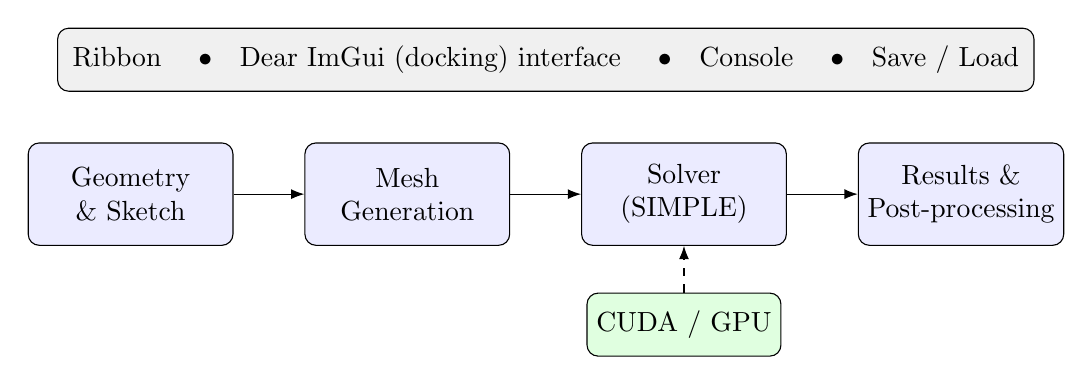
\begin{tikzpicture}[>=Latex,
  stage/.style={draw, rounded corners, minimum width=26mm, minimum height=13mm, align=center, fill=blue!8},
  band/.style={draw, rounded corners, align=center, fill=gray!12, minimum height=8mm}]
  \node[stage](sk){Geometry\\ \& Sketch};
  \node[stage, right=9mm of sk](me){Mesh\\ Generation};
  \node[stage, right=9mm of me](so){Solver\\ (SIMPLE)};
  \node[stage, right=9mm of so](re){Results \&\\ Post-processing};
  \draw[->](sk)--(me); \draw[->](me)--(so); \draw[->](so)--(re);
  \node[band, minimum width=124mm] at ($(sk.north)!0.5!(re.north)+(0,1.05)$)
      {Ribbon \quad$\bullet$\quad Dear ImGui (docking) interface \quad$\bullet$\quad Console \quad$\bullet$\quad Save / Load};
  \node[band, fill=green!12] at ($(so.south)+(0,-1.0)$) (gpu){CUDA / GPU};
  \draw[->,dashed](gpu)--(so);
\end{tikzpicture}
\caption{High-level architecture. A shared project flows left to right through four
stages; the ribbon, GUI and console wrap all stages, and the solver offloads to the GPU.}
\label{fig:arch}
\end{figure}

This manual documents the most notable features. Because AxiSim is under active
development, some smaller features may be described only briefly, and details are
subject to change between versions.

% ======================================================================
\section{Disclaimers and Project Status}\label{sec:disclaimer}
% ======================================================================
\warnbox{\textbf{AxiSim is alpha-stage, work-in-progress software. Its numerical results
have not been formally verified or validated. Do not use it for engineering decisions,
safety-critical work, or any application where correctness matters.}}

\subsection{Development status}
AxiSim is at version \texttt{1.05-alpha}. It is updated frequently and changes rapidly;
APIs, file formats, default parameters, and behaviour may change without notice between
versions. Expect rough edges, incomplete features, and the occasional bug.

\subsection{Verification and validation}
The solver has \emph{not} undergone systematic verification (e.g.\ method-of-manufactured-
solutions, grid-convergence studies) or validation against analytical solutions,
trusted reference codes, or experimental data. Results should be treated as
qualitative and exploratory. Known numerical caveats are collected in
Section~\ref{sec:limitations}.

\warnbox{\textbf{Results produced before v1.05-alpha may be quantitatively wrong.} Two
corrections landed in this cycle that change converged solutions rather than only their
speed: the concentration mass flux no longer multiplies by density twice
(Section~\ref{sec:scalars}), and the face flux at a fixed-pressure boundary now carries
its Rhie--Chow pressure term (Section~\ref{sec:rhiechow}). Cases driven by a prescribed
pressure difference, and any case with concentration transport, should be re-run.}

\subsection{Intended use}
AxiSim is intended for learning, prototyping, and experimentation with FVM/CFD and
GPU programming. It is not a substitute for a validated commercial or open-source
solver.

\subsection{Licensing}
The original AxiSim source code is released under the MIT License. However, AxiSim
links the \textbf{Gmsh} library, which is licensed under the GNU GPL v2-or-later.
\emph{Binaries that are built with and distributed alongside Gmsh are therefore
subject to the GPL}, in addition to the MIT terms covering AxiSim's own source. The
third-party components and their licenses are listed in Section~\ref{sec:libraries}.

% ======================================================================
\section{System Requirements and Installation}
% ======================================================================
\subsection{Requirements}
\begin{itemize}[nosep]
  \item \textbf{Operating system:} Windows 10 / 11 (x64).
  \item \textbf{GPU:} an NVIDIA GPU with CUDA compute capability \(\geq 7.5\)
        (Turing / GTX 16 / RTX 20 series and newer) plus a recent driver. AxiSim runs
        its solver on the GPU and \emph{will not run} on machines without a compatible
        NVIDIA card. Release builds must be compiled for the GPU architectures they
        are expected to support.
  \item \textbf{To build from source:} CUDA Toolkit 13.0, a C++20 compiler
        (Visual Studio 2022), CMake \(\geq 3.24\), Ninja, and vcpkg.
\end{itemize}

\subsection{Building from source}
Dependencies that come from vcpkg (GLFW, GLAD, GLM, OpenGL) are installed first; Gmsh
and Dear ImGui/ImPlot are bundled in the repository. The repository currently includes
\texttt{CMakeSettings.json} for Visual Studio's CMake integration. If configuring from
the command line, use the vcpkg toolchain file explicitly:
\begin{lstlisting}[language={}]
vcpkg install glfw3 glad glm
cmake -S . -B out/build/x64-Release -G Ninja ^
  -DCMAKE_BUILD_TYPE=RelWithDebInfo ^
  -DCMAKE_TOOLCHAIN_FILE=<path-to-vcpkg>/scripts/buildsystems/vcpkg.cmake
cmake --build out/build/x64-Release --target AxiSim
\end{lstlisting}

\warnbox{\textbf{CUDA architecture note.} The checked-in CMake file currently targets
\texttt{CUDA\_ARCHITECTURES "86-real"} for a local Ampere development GPU. For a
redistributable build, change this list to include the architectures you intend to
support (for example Turing/Ampere/Ada plus a PTX fallback). Otherwise the produced
binary may only run on matching GPUs even though the source code targets CUDA-capable
hardware more broadly.}

\subsection{Runtime files}
The executable loads several resources by relative path, so the following must sit
next to \texttt{AxiSim.exe} when distributing or running outside the build tree:
\texttt{glfw3.dll}, \texttt{gmsh-4.15.dll}, the \texttt{assets/} folder (fonts and
icons), and the \texttt{graphics/shaders/} folder. The CUDA runtime is statically
linked, so end users do not need the CUDA Toolkit---only an NVIDIA driver. The Visual
C++ runtime (\texttt{MSVCP140.dll}, \texttt{VCRUNTIME140*.dll}) must be present (install
the Microsoft Visual C++ Redistributable x64 if needed).

\subsection{Packaging a release ZIP}
The \texttt{package.ps1} script builds the \texttt{AxiSim} target, installs it into a
staging directory, checks for required runtime assets, and writes a ZIP under
\texttt{dist/}. A typical release-package command is:
\begin{lstlisting}[language={}]
.\package.ps1 -Version v1.05-alpha
\end{lstlisting}
Use \texttt{-SkipBuild} only when the chosen build directory already contains a fresh
successful build. The package still cannot include the user's NVIDIA driver; target
machines need a compatible driver and GPU.

% ======================================================================
\section{Libraries and Dependencies}\label{sec:libraries}
% ======================================================================
Table~\ref{tab:libs} lists the notable external components used by AxiSim.

\begin{table}[h]
\centering
\caption{External libraries and their roles.}
\label{tab:libs}
\begin{tabular}{@{}>{\raggedright\arraybackslash}p{0.20\linewidth}
                   >{\raggedright\arraybackslash}p{0.52\linewidth}
                   >{\raggedright\arraybackslash}p{0.20\linewidth}@{}}
\toprule
\textbf{Library} & \textbf{Role in AxiSim} & \textbf{License} \\
\midrule
OpenGL              & Graphics API for creating the window and rendering models       & system \\
GLSL                & Shading language used with OpenGL to render onto the screen      & (OpenGL) \\
GLFW                & Window creation, OS context, and input handling                  & zlib/libpng \\
GLAD                & OpenGL function loader                                            & MIT/public \\
GLM                 & Vector / matrix / quaternion math (camera, transforms)           & MIT \\
Dear ImGui (docking)& Main GUI library; docking branch for dockable windows           & MIT \\
ImPlot              & Real-time plotting (residual plots)                              & MIT \\
Gmsh                & Unstructured (triangular) mesh generation                        & \textbf{GPL v2+} \\
stb\_image          & Loading PNG icon/texture assets                                  & MIT/public \\
NVIDIA CUDA Toolkit & GPU compute: assembly, linear solvers, multigrid, CUDA graphs    & NVIDIA EULA \\
\bottomrule
\end{tabular}
\end{table}

\noindent See Section~\ref{sec:disclaimer} for the licensing consequence of linking Gmsh.

% ======================================================================
\section{What Is Included: Application Overview}
% ======================================================================
AxiSim ships as a single application whose major components are:
\begin{itemize}[nosep]
  \item \textbf{Geometry / Sketch view} --- draw the axisymmetric cross-section
        (lines, rectangles, circles, arcs) with live dimensions, snapping, trim,
        erase, select/move, copy/paste, and undo/redo.
  \item \textbf{Mesh Inspector} --- convert the sketch into a structured (Cartesian
        or multi-block) or unstructured (Gmsh) mesh, define boundary groups, add local
        refinement regions, and inspect per-cell mesh data.
  \item \textbf{Solver} --- configure and run the SIMPLE solver; choose discretisation
        schemes, relaxation, linear solver and multigrid, steady/transient mode, and
        optional scalar transport.
  \item \textbf{Results} --- 3D revolved field visualisation and a 2D cross-section
        inspector with colormaps, a colorbar, optional mirroring about the axis, and
        transient animation playback.
  \item \textbf{Console} --- text commands to drive major operations and settings.
  \item \textbf{Residual plot} --- live convergence monitoring via ImPlot.
  \item \textbf{Save / Load} --- persist and reload project state, including results,
        through the File menu or console commands.
\end{itemize}

A typical end-to-end session follows the workflow in Figure~\ref{fig:workflow}.

\begin{figure}[h]
\centering
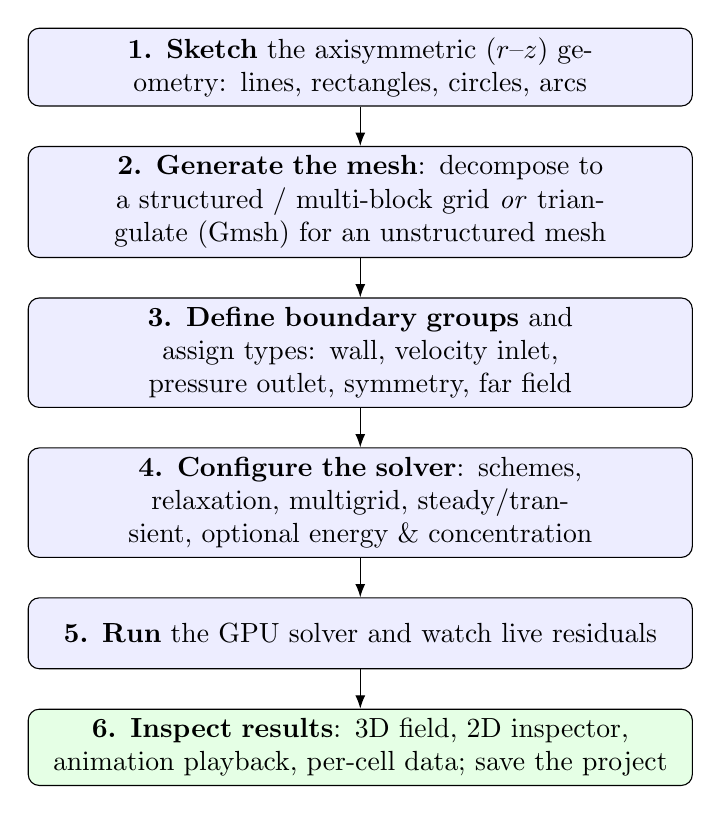
\begin{tikzpicture}[>=Latex, node distance=5mm,
  wfbox/.style={draw, rounded corners, align=center, text width=82mm, minimum height=9mm, fill=blue!7}]
  \node[wfbox](s1){\textbf{1. Sketch} the axisymmetric ($r$--$z$) geometry: lines, rectangles, circles, arcs};
  \node[wfbox, below=of s1](s2){\textbf{2. Generate the mesh}: decompose to a structured / multi-block grid \emph{or} triangulate (Gmsh) for an unstructured mesh};
  \node[wfbox, below=of s2](s3){\textbf{3. Define boundary groups} and assign types: wall, velocity inlet, pressure outlet, symmetry, far field};
  \node[wfbox, below=of s3](s4){\textbf{4. Configure the solver}: schemes, relaxation, multigrid, steady/transient, optional energy \& concentration};
  \node[wfbox, below=of s4](s5){\textbf{5. Run} the GPU solver and watch live residuals};
  \node[wfbox, below=of s5, fill=green!10](s6){\textbf{6. Inspect results}: 3D field, 2D inspector, animation playback, per-cell data; save the project};
  \foreach \a/\b in {s1/s2,s2/s3,s3/s4,s4/s5,s5/s6}{\draw[->](\a)--(\b);}
\end{tikzpicture}
\caption{The typical AxiSim workflow.}
\label{fig:workflow}
\end{figure}

% ======================================================================
\section{Interface Layout and Units}\label{sec:ui}
% ======================================================================
\subsection{Window layout}
The application window is arranged as a fixed top band, a dockspace, and a status bar:

\begin{itemize}[nosep]
  \item \textbf{Menu bar} --- File, Edit, and View menus.
  \item \textbf{Ribbon} --- a single application-wide toolbar strip beneath the menu
        bar. It is context sensitive: each tab contributes its own tool groups
        (clipboard, home/reset view, create, edit, view), separated into named groups.
        Before v1.05 these tools lived inside each viewport panel.
  \item \textbf{Project panel} --- the four setup tabs (Geometry, Mesh, Solver,
        Results), each showing a navigation tree and a primary action button
        (\textbf{Generate Mesh}, \textbf{Start Solver}, \textbf{Generate Results}).
  \item \textbf{Overview panel} --- the properties panel for whatever is selected in
        the tree.
  \item \textbf{Viewport} --- the sketch view, mesh inspector, residual plot, or
        results scene, depending on the active tab.
  \item \textbf{Console} --- docked beneath the setup tabs.
  \item \textbf{Status bar} --- ready/busy indicator, the current project name, and the
        active length unit.
\end{itemize}

\textbf{View \(\rightarrow\) GUI} toggles \emph{simple view}, which hides every panel
except the live viewport (setup tabs, console, ribbon, and status bar all disappear) so
the field fills the window. Toggling it back restores the previous layout.

\subsection{Units}\label{sec:units}
v1.05-alpha introduces a project-wide unit system. All values are stored internally in
base SI units; conversion happens only at the user-interface edge, so changing a display
unit never changes the solution.

Units are edited in one place: \textbf{Edit \(\rightarrow\) Units}, which opens a modal
listing every quantity and its available units. Elsewhere in the interface the unit is
shown as read-only text next to the value it belongs to. A single project-wide
\emph{length scale} governs geometry, mesh, sketch dimensions, and wall-layer thickness,
and is echoed in the status bar (for example \texttt{Units: mm}).

\begin{table}[h]
\centering
\caption{Unit families and the options offered for each. The first entry of each row is
the internal base unit.}
\label{tab:units}
\begin{tabular}{@{}>{\raggedright\arraybackslash}p{0.26\linewidth}
                   >{\raggedright\arraybackslash}p{0.66\linewidth}@{}}
\toprule
\textbf{Quantity} & \textbf{Units} \\
\midrule
Length            & m, cm, mm, \(\mu\)m \\
Velocity          & m/s, mm/s, cm/s, \(\mu\)m/s \\
Pressure          & Pa, kPa, MPa, bar, kg\,m\(^{-1}\)s\(^{-2}\), atm \\
Temperature       & K, \(^\circ\)C, \(^\circ\)F (offset units) \\
Density           & kg/m\(^3\), kg/mm\(^3\) \\
Dynamic viscosity & Pa\,s, kg\,m\(^{-1}\)s\(^{-1}\), kg\,mm\(^{-1}\)s\(^{-1}\), mPa\,s \\
Specific heat     & J/(kg\,K), kJ/(kg\,K), J/(g\,K), cal/(g\,K) \\
Thermal conductivity & W/(m\,K), W/(cm\,K), W/(mm\,K), mW/(mm\,K) \\
Diffusivity       & m\(^2\)/s, mm\(^2\)/s, cm\(^2\)/s, \(\mu\)m\(^2\)/s \\
Concentration     & nmol/m\(^3\), mol/m\(^3\), M, mM, \(\mu\)M, nM, nmol/mL, nmol/mm\(^3\) \\
Reaction rate \(V_{\max}\) & nmol/(m\(^2\)s), mol/(m\(^2\)s), \(\mu\)mol/(m\(^2\)s), pmol/(m\(^2\)s), nmol/(cm\(^2\)s), nmol/(mm\(^2\)s) \\
Time              & s, min \\
\bottomrule
\end{tabular}
\end{table}

% ======================================================================
\section{Getting Started: A Typical Workflow}
% ======================================================================
\subsection{Sketching the geometry}
The geometry view lets you draw the cross-section of the axisymmetric domain in the
\((z, r)\) half-plane. Supported primitives are lines, rectangles, circles, and arcs,
with live dimensioning and snapping to existing geometry, grid vertices, and the origin.
The ribbon provides reset-view, dimension, trim, erase, line, rectangle, circle, grid
display, screenshot, and clipboard controls. Selection supports single clicks, box
selection, moving selected segments, copy/paste, undo/redo, and editable dimension
labels. The Geometry panel also lists sketch entities so they can be selected and
deleted from the tree. A 2D camera (pan with the middle mouse button, zoom with the
wheel) frames the sketch; the background grid and its spacing legend are shown by
default.

\notebox{\textbf{Changed in v1.05-alpha.} The two axis \emph{lines} (\(r=0\) and \(z=0\))
are no longer snap candidates. They span the whole canvas, so anything drawn near an
axis was pulled onto it. The origin remains snappable, as do vertices and geometry.}

\begin{figure}[h]
\centering
\screenshot{ui_sketch.png}{0.92\linewidth}{geometry sketching view}
\caption{Sketching the axisymmetric cross-section. The ribbon above the dockspace
carries the clipboard, view, create, and edit tools for the active tab.}
\label{fig:sketch}
\end{figure}

\subsection{Generating the mesh}
With a closed sketch, the Mesh Inspector converts the geometry into a finite-volume
mesh (Section~\ref{sec:mesh}). Choose either a structured or an unstructured mesh in the
Mesh tab, then press \textbf{Generate Mesh}. The Statistics panel reports the mesh type
and the resulting cell and node counts. Boundary segments are detected automatically and
can be grouped and named for boundary-condition assignment. If no sketch geometry
exists, the mesh generator falls back to a simple default domain so the rest of the
workflow can still be exercised.

\subsection{Defining boundaries and running}
Assign a boundary type to each named group, configure the solver
(Section~\ref{sec:solver}), and run. The residual plot updates live so you can monitor
convergence. When the run finishes, switch to the Results tab to explore the field.

\subsection{Saving the project}
Use \textbf{File \(\rightarrow\) Save}, \textbf{File \(\rightarrow\) Save As}, or
\texttt{save project} in the console to persist the whole project, including its
results. Use \textbf{File \(\rightarrow\) Open \(\rightarrow\) Project} or
\texttt{load project} to reload it. The File menu can also mark the current project as
the one to reopen at startup, and can import or export the geometry on its own.

% ======================================================================
\section{Mesh Generation}\label{sec:mesh}
% ======================================================================
AxiSim supports three meshing paths---single-block structured, multi-block structured,
and unstructured---all reduced to a common finite-volume representation
(Section~\ref{sec:fvdata}).

\subsection{Structured mesh}
The structured mesh is a Cartesian grid in the \((z, r)\) plane defined by the number of
cells \(n_z\) and \(n_r\), the domain length \(L\) and radius \(R\), and optional axial/
radial grading (\texttt{zBias}, \texttt{rBias}). The sketch is \emph{rasterised} onto this
grid: every cell whose centre lies outside the sketched domain (or inside an obstacle)
is flagged solid. This is recorded in \texttt{activeCell} (1 = fluid, 0 = solid) and the
set \texttt{obstacleIndices}. Cell index ordering is row-major, \(n = i\,n_z + j\), where
\(i\) is the radial index and \(j\) the axial index.

\subsection{Multi-block structured mesh}\label{sec:multiblock}
\notebox{\textbf{New in v1.05-alpha.} A sketch made of axis-aligned rectilinear geometry
is now decomposed into conformal structured blocks instead of being rasterised onto one
grid.}

Multi-block generation uses a \emph{trellis} decomposition. Every distinct \(z\) and
\(r\) coordinate in the sketch becomes a grid line; the lines cut the bounding box into
a lattice of rectangles, and each rectangle whose centre lies inside the fluid domain
becomes one block (Figure~\ref{fig:trellis}). Obstacles are simply the rectangles whose
centres fall outside the domain, so they are omitted rather than flagged solid.

Resolution is controlled per \emph{band} rather than per block: \texttt{zBandCells} holds
the axial cell count for each gap between consecutive \(z\) lines, and
\texttt{rBandCells} the radial count for each \(r\) band. Because neighbouring blocks
share a band's cell count, every block seam is conformal by construction---there are no
hanging nodes and no interpolation across block interfaces.

\begin{figure}[h]
\centering
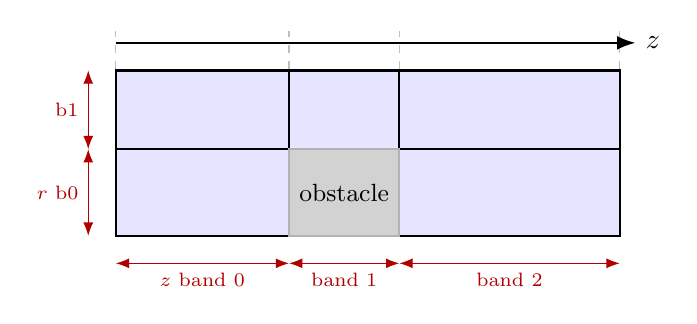
\begin{tikzpicture}[scale=1.0, >=Latex]
  % trellis lines
  \draw[gray!50, dashed] (0,0) -- (0,2.6);
  \draw[gray!50, dashed] (2.2,0) -- (2.2,2.6);
  \draw[gray!50, dashed] (3.6,0) -- (3.6,2.6);
  \draw[gray!50, dashed] (6.4,0) -- (6.4,2.6);
  \draw[gray!50, dashed] (0,0) -- (6.4,0);
  \draw[gray!50, dashed] (0,1.1) -- (6.4,1.1);
  \draw[gray!50, dashed] (0,2.1) -- (6.4,2.1);
  % blocks
  \fill[blue!10] (0,0) rectangle (2.2,1.1);
  \fill[blue!10] (0,1.1) rectangle (2.2,2.1);
  \fill[blue!10] (2.2,1.1) rectangle (3.6,2.1);
  \fill[blue!10] (3.6,0) rectangle (6.4,1.1);
  \fill[blue!10] (3.6,1.1) rectangle (6.4,2.1);
  \fill[gray!35] (2.2,0) rectangle (3.6,1.1);
  \draw[thick] (0,0) rectangle (2.2,1.1);
  \draw[thick] (0,1.1) rectangle (2.2,2.1);
  \draw[thick] (2.2,1.1) rectangle (3.6,2.1);
  \draw[thick] (3.6,0) rectangle (6.4,1.1);
  \draw[thick] (3.6,1.1) rectangle (6.4,2.1);
  \draw[thick, gray!60] (2.2,0) rectangle (3.6,1.1);
  \node at (2.9,0.55) {\small obstacle};
  % band labels
  \draw[<->, red!70!black] (0,-0.35) -- (2.2,-0.35) node[midway,below]{\scriptsize $z$ band 0};
  \draw[<->, red!70!black] (2.2,-0.35) -- (3.6,-0.35) node[midway,below]{\scriptsize band 1};
  \draw[<->, red!70!black] (3.6,-0.35) -- (6.4,-0.35) node[midway,below]{\scriptsize band 2};
  \draw[<->, red!70!black] (-0.35,0) -- (-0.35,1.1) node[midway,left,rotate=0]{\scriptsize $r$ b0};
  \draw[<->, red!70!black] (-0.35,1.1) -- (-0.35,2.1) node[midway,left]{\scriptsize b1};
  \draw[->, thick] (0,2.45) -- (6.6,2.45) node[right]{$z$};
\end{tikzpicture}
\caption{Trellis decomposition. Each distinct sketch coordinate becomes a grid line;
interior rectangles become conformal blocks and exterior ones are dropped as obstacles.
Cell counts are stored per band, so blocks sharing a band always match across the seam.}
\label{fig:trellis}
\end{figure}

The multi-block path is only taken when the sketch is representable by it. Circles,
arcs, skewed (non-axis-aligned) outline edges, open line loops, and degenerate
rectangles are rejected with a user-facing reason, and the mesher falls back to the
rasterised single-block grid. Multi-block state is derived from the sketch rather than
serialised, so it is rebuilt after a project load.

Because the results pipeline is raster based---it revolves \texttt{g.zFace}/
\texttt{g.rFace} and samples a raster texture---a multi-block solution is resampled onto
the raster grid before display, through a raster-to-cell map built once per generation.

\subsection{Unstructured mesh}
The unstructured mesh is a constrained Delaunay triangulation produced by Gmsh from the
sketch boundary. Local refinement is controlled by \emph{regions of influence}
(rectangular or circular), which set a target element size inside the region and a
transition to the background size outside it. Boundary sizing (edge count / target
spacing / bias) can be set per boundary segment or group. Each triangle becomes one
finite-volume cell. Sketch rectangles, circles, and arcs are sampled into boundary
segments before triangulation; the outermost closed loop is treated as the domain and
inner loops become obstacles.

\begin{figure}[h]
\centering
\begin{subfigure}{0.48\linewidth}\centering
  \screenshot{mesh_structured.png}{\linewidth}{structured mesh}
  \caption{Structured (Cartesian) mesh.}
\end{subfigure}\hfill
\begin{subfigure}{0.48\linewidth}\centering
  \screenshot{mesh_unstructured.png}{\linewidth}{unstructured mesh}
  \caption{Unstructured (Gmsh) mesh.}
\end{subfigure}
\caption{The two meshing families.}
\label{fig:meshes}
\end{figure}

\begin{figure}[h]
\centering
\screenshot{ui_mesh.png}{0.92\linewidth}{mesh tab with statistics}
\caption{The Mesh tab. The Statistics panel reports the mesh type and the generated cell
and node counts; the boundary tree lists the named groups.}
\label{fig:meshtab}
\end{figure}

\subsection{Finite-volume data structure}\label{sec:fvdata}
Regardless of mesh family, the solver consumes a single \texttt{FVMesh} made of cells and
faces. A cell stores its centroid, 2D area, revolved volume \(V = 2\pi r_c A_{2D}\)
(axisymmetric), and the IDs of its bounding faces. A face stores its owner and neighbour
cell, its outward unit normal, its centre, and its (revolved) area; a face with
\texttt{neighbor} \(= -1\) is a boundary face.

\begin{lstlisting}
struct FVCell {
    Vec2 center;          // centroid (z, r)
    double area2D = 0.0;  // 2D cross-sectional area
    double volume = 0.0;  // revolved volume 2*pi*r_c*area2D
    std::vector<int> faceIDs;
    bool active = true;   // false => solid / excluded
    bool solid  = false;
};

struct FVFace {
    int owner = -1, neighbor = -1;  // neighbor < 0  => boundary face
    int v0 = -1, v1 = -1;           // edge endpoints
    Vec2 normal, center;            // outward unit normal; face midpoint
    double length2D = 0.0, area = 0.0;
    int boundaryGroupID = -1;
};
\end{lstlisting}

\noindent \texttt{area2D} is now populated on every path (structured, multi-block, and
unstructured), since the cell Reynolds number derived in Section~\ref{sec:derived} reads
it as the cell length scale.

Figure~\ref{fig:fvcell} shows two adjacent (triangular) cells, the owner $P$ and
neighbour $N$, the centroid-to-centroid vector $\mathbf{d}$, and the face outward
normal $\mathbf{S}$. These two quantities drive both the diffusion discretisation and
the mesh-quality measure below.

\begin{figure}[h]
\centering
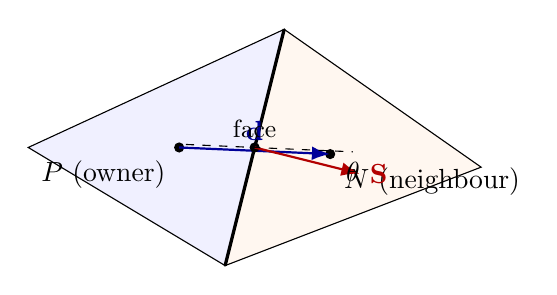
\begin{tikzpicture}[>=Latex, scale=1.25,
  dot/.style={circle, fill=black, inner sep=1.3pt}]
  \coordinate (F1) at (2,0);
  \coordinate (F2) at (2.6,2.4);
  \coordinate (PL) at (0,1.2);
  \coordinate (NR) at (4.6,1.0);
  \draw[fill=blue!6]   (F1)--(F2)--(PL)--cycle;
  \draw[fill=orange!6] (F1)--(F2)--(NR)--cycle;
  \draw[very thick] (F1)--(F2);
  \coordinate (P) at (1.533,1.2);
  \coordinate (N) at (3.067,1.133);
  \node[dot,label=below left:{$P$ (owner)}] at (P){};
  \node[dot,label=below right:{$N$ (neighbour)}] at (N){};
  \draw[->,thick,blue!60!black] (P)--(N) node[midway,above]{$\mathbf{d}$};
  \coordinate (Fm) at (2.3,1.2);
  \node[dot] at (Fm){};
  \draw[->,thick,red!70!black] (Fm)--($(Fm)+(1.066,-0.266)$) node[right]{$\mathbf{S}$};
  \draw[dashed] (1.601,1.231)--(3.299,1.156);
  \node at (3.30,0.95){$\theta$};
  \node[above] at (Fm){\small face};
\end{tikzpicture}
\caption{Two adjacent finite-volume cells. $\mathbf{d}$ joins the cell centroids and
$\mathbf{S}$ is the shared-face outward normal. The angle $\theta$ between them is the
\emph{non-orthogonality} (zero for a perfectly orthogonal mesh).}
\label{fig:fvcell}
\end{figure}

\subsection{Boundary groups}
Boundary faces are organised into named \emph{boundary groups}. Domain edges and
obstacle edges are detected, merged into segments, and the user groups and names them.
Each group carries a boundary type and per-field values that the solver reads when
applying boundary conditions (Section~\ref{sec:bc}). Groups also store orientation
metadata, total boundary length, optional boundary sizing, and optional scalar wall
layers. For structured meshes, groups retain a lookup to their grid edges; for
unstructured meshes, groups are resolved through boundary vertices, edges, and
segments. On the multi-block path, external block faces are classified into groups by
geometric match against the sketch-derived boundary edges.

\notebox{\textbf{Changed in v1.05-alpha.} Boundary group IDs are allocated from a
monotonic counter that is never rewound while a project is open. Previously an ID was
taken as \(\max(\text{id})+1\) over the live group vector, so re-meshing---which rebuilds
that vector---handed retired IDs back out to different boundaries, and a selection held
across the rebuild could silently resolve to an unrelated group. Projects saved before
this change are migrated on load.}

\subsection{Regions of influence}
Regions of influence are local mesh-sizing controls for unstructured meshes. A region
may be circular or rectangular, enabled/disabled independently, and configured with a
target spacing, outside spacing, and transition thickness. v1.05-alpha adds an
\texttt{overrideBoundarySpacing} flag so a region can take precedence over the boundary
sizing of any segment it covers---useful when a refinement box crosses a boundary that
was given a coarser spacing of its own. Regions are saved with the project.

\subsection{Mesh quality: non-orthogonality}\label{sec:nonortho}
For each interior face, the non-orthogonality angle is
\begin{equation}
\theta = \arccos\!\left(\frac{\mathbf{d}\cdot\mathbf{S}}{\lvert\mathbf{d}\rvert\,\lvert\mathbf{S}\rvert}\right),
\end{equation}
where $\mathbf{d}$ is the owner-to-neighbour centroid vector and $\mathbf{S}$ the face
normal. A value of $0^\circ$ means the centroid line is parallel to the face normal
(ideal); larger angles increase discretisation error and can slow or destabilise the
solve. The Mesh Inspector's cell-pick tool reports each cell's centroid, area/volume,
face count, per-face neighbour and length, and the per-cell maximum and average
non-orthogonality. Structured and multi-block cells report $\approx 0^\circ$ (a useful
sanity check), while skewed triangles report larger values.

% ======================================================================
\section{Solver}\label{sec:solver}
% ======================================================================
\subsection{Governing equations}
AxiSim solves the steady or unsteady incompressible Navier--Stokes equations in
axisymmetric \((z, r)\) coordinates (no swirl). Continuity and momentum are
\begin{align}
\frac{\partial u_z}{\partial z} + \frac{1}{r}\frac{\partial (r\,u_r)}{\partial r} &= 0, \\[4pt]
\rho\,\frac{D u_z}{Dt} &= -\frac{\partial p}{\partial z}
   + \mu\!\left[\frac{\partial^2 u_z}{\partial z^2} + \frac{1}{r}\frac{\partial}{\partial r}\!\left(r\,\frac{\partial u_z}{\partial r}\right)\right], \\[4pt]
\rho\,\frac{D u_r}{Dt} &= -\frac{\partial p}{\partial r}
   + \mu\!\left[\frac{\partial^2 u_r}{\partial z^2} + \frac{\partial}{\partial r}\!\left(\frac{1}{r}\frac{\partial (r\,u_r)}{\partial r}\right)\right].
\end{align}
Optional passive scalars---temperature \(T\) (energy) and concentration \(C\)---are
transported by convection--diffusion equations and can be enabled independently
(\texttt{solveEnergy}, \texttt{solveConcentration}). The scalars are solved after the
momentum/pressure update within the SIMPLE iteration. The concentration solver also
supports reactive wall-consumption boundary conditions.

\subsection{Scalar transport and wall reactions}\label{sec:scalars}
The scalar equations use the same finite-volume mesh and optional convection term as
the momentum equations. In compact form:
\begin{align}
\frac{\partial T}{\partial t} + \nabla\cdot(\mathbf{u}T)
  &= \nabla\cdot(\alpha_T\nabla T), \qquad
     \alpha_T = \frac{k}{\rho c_p}, \\
\frac{\partial C}{\partial t} + \nabla\cdot(\mathbf{u}C)
  &= \nabla\cdot(D\nabla C).
\end{align}

\warnbox{\textbf{Corrected in v1.05-alpha.} The concentration convection term was
building its face flux from the momentum mass flux \(\dot m = \rho\,\mathbf{u}\cdot
\mathbf{S}\) and then multiplying by density a second time. Concentration transport is
volumetric---the correct face flux is \(\mathbf{u}\cdot\mathbf{S}\)---so every converged
concentration field produced before this fix was scaled by an extra factor of \(\rho\)
in its convective balance. Concentration results from earlier versions should be
discarded and re-run.}

For concentration walls, Michaelis--Menten and Hill kinetic conditions are available.
The wall concentration \(C_w\) is found from a transfer balance between the cell value
\(C_P\), the cell-to-face diffusion resistance, any user-entered wall-layer resistance,
and the reaction flux:
\begin{equation}
h(C_P - C_w) = J(C_w).
\end{equation}
For Michaelis--Menten kinetics,
\begin{equation}
J_{MM}(C_w)=\frac{V_{\max} C_w}{K_m + C_w}\,I(C_w),
\end{equation}
and for Hill kinetics,
\begin{equation}
J_H(C_w)=\frac{V_{\max} C_w^n}{K_m^n + C_w^n}\,I(C_w).
\end{equation}
The optional inhibition factor is
\begin{equation}
I(C_w)=1-\frac{V_2 C_w^m}{K_2^m + C_w^m},
\end{equation}
and is disabled by setting \(V_2=0\). The solver uses Newton iterations on the GPU to
solve the wall balance and clamps negative wall concentrations to zero.

\subsection{The SIMPLE algorithm}
Pressure--velocity coupling uses SIMPLE (Semi-Implicit Method for Pressure-Linked
Equations). Each outer iteration solves under-relaxed momentum predictors, then a
pressure-correction equation, then corrects velocity, pressure, and the face mass flux
(Figure~\ref{fig:simple}). Under-relaxation is required for stability; the defaults are
momentum \(\approx 0.7\) and pressure \(\approx 0.3\).

\begin{figure}[h]
\centering
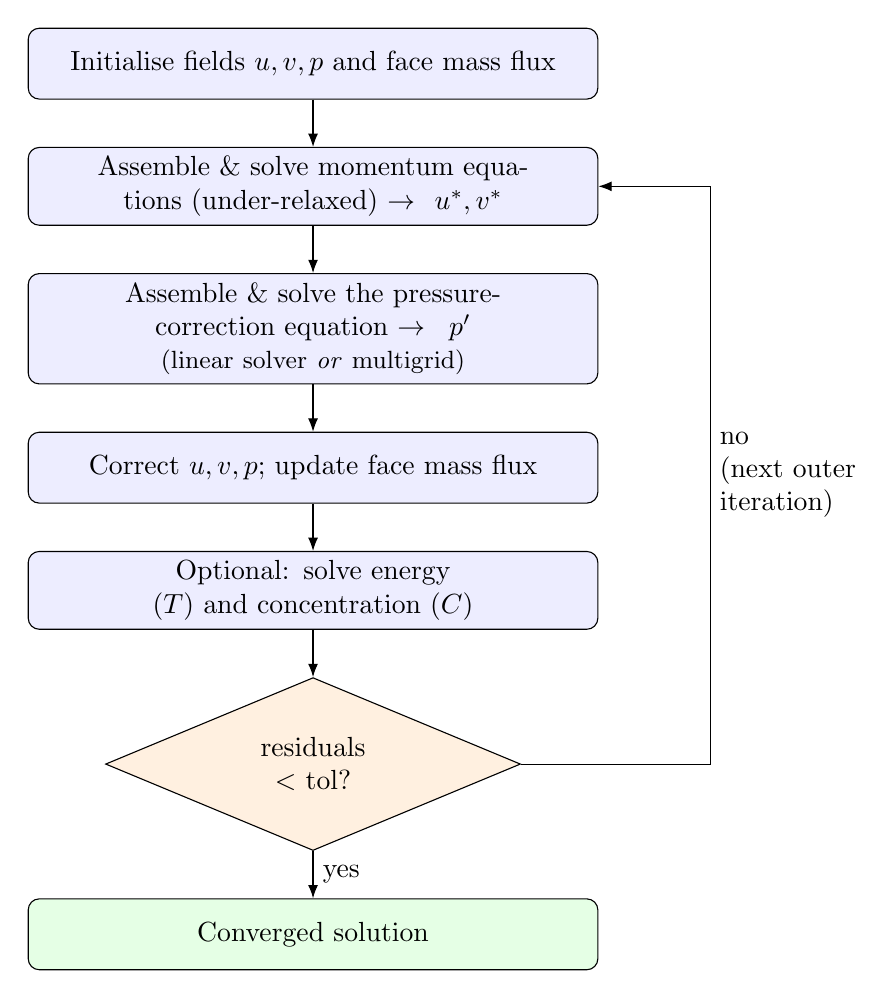
\begin{tikzpicture}[>=Latex, node distance=6mm,
  box/.style={draw, rounded corners, align=center, text width=70mm, minimum height=9mm, fill=blue!7},
  dec/.style={draw, diamond, aspect=2.4, align=center, fill=orange!12, inner sep=1pt, text width=34mm}]
  \node[box](init){Initialise fields $u,v,p$ and face mass flux};
  \node[box,below=of init](mom){Assemble \& solve momentum equations (under-relaxed) $\rightarrow u^{*}, v^{*}$};
  \node[box,below=of mom](pp){Assemble \& solve the pressure-correction equation $\rightarrow p'$ \\ \small(linear solver \emph{or} multigrid)};
  \node[box,below=of pp](corr){Correct $u, v, p$; update face mass flux};
  \node[box,below=of corr](scal){Optional: solve energy ($T$) and concentration ($C$)};
  \node[dec,below=of scal](conv){residuals\\ $<$ tol?};
  \node[box,below=of conv, fill=green!10](done){Converged solution};
  \draw[->](init)--(mom); \draw[->](mom)--(pp); \draw[->](pp)--(corr);
  \draw[->](corr)--(scal); \draw[->](scal)--(conv);
  \draw[->](conv)--node[right]{yes}(done);
  \draw[->](conv.east) -- ++(2.4,0) |- node[pos=0.25,right,align=left]{no\\ (next outer\\ iteration)} (mom.east);
\end{tikzpicture}
\caption{One outer iteration of the SIMPLE loop as implemented in AxiSim.}
\label{fig:simple}
\end{figure}

\subsection{Rhie--Chow interpolation at boundaries}\label{sec:rhiechow}
Face velocities are reconstructed with Rhie--Chow momentum interpolation, which adds to
the linearly interpolated face velocity a compact pressure difference minus the smooth
cell-centred gradient:
\begin{equation}
u_n = u_n^{\text{lin}} - D_f\!\left(\frac{p_N - p_P}{\lvert\mathbf{d}\rvert}
      - \overline{\nabla p}\cdot\hat{\mathbf{n}}\right).
\end{equation}

\warnbox{\textbf{Corrected in v1.05-alpha.} This correction was previously skipped on
\emph{all} boundary faces, so the flux at a pressure outlet was \(\rho A\,\mathbf{u}_P
\cdot\hat{\mathbf{n}}\) with no pressure dependence---while the pressure-correction
equation already assembled the matching sensitivity \(\partial\dot m_b/\partial p_P\) for
that same face. The two halves of SIMPLE were therefore inconsistent, and a case driven
purely by a prescribed pressure difference never felt its outlet pressure except through
the momentum body force. The correction is now applied on fixed-pressure (Dirichlet)
boundary faces, with the boundary face standing in for the neighbour cell. Other
boundary types carry zero-gradient pressure and are deliberately left untouched, since
adding a pressure term there would inject a flux the \(p'\) equation does not account
for.}

\subsection{Discretisation schemes}
Equations are discretised with the finite-volume method. The \emph{convection} schemes
exposed in the GUI are first-order upwind, central differencing, and second-order
upwind. Diffusion uses the centroid-distance gradient along $\mathbf{d}$ plus an
optional \emph{non-orthogonal correction} for the cross term
(Section~\ref{sec:nonortho}), toggled by \texttt{useNonOrthCorrector} (default off,
i.e.\ orthogonal-only, which is the stable default). The option is disabled on a
structured mesh, which is orthogonal by construction and so has no cross term to
correct. The cell-gradient scheme used for the pressure and pressure-correction
gradients is selectable in the Solver panel as \textbf{Pressure Gradient}: Green--Gauss
or Least Squares.

\subsection{Linear solvers}\label{sec:linear}
The discretised systems are solved on the GPU. The GUI exposes \textbf{Jacobi} and
\textbf{red--black Gauss--Seidel} for the main SIMPLE solve, plus an independent
\textbf{Multigrid} toggle that replaces the linear solver for the pressure correction
only (Section~\ref{sec:multigrid}). Inner iteration counts, SIMPLE iteration counts,
residual frequency, and tolerances are configurable through the solver settings.

\notebox{\textbf{New in v1.05-alpha.} Gauss--Seidel is no longer structured-only. It used
to take its checkerboard ordering from \((i+j)\bmod 2\), which requires a real
\(n_r\times n_z\) grid; on the face-based path (multi-block and unstructured)
\(n_r=n_z=0\) and that kernel divided by zero. The ordering now comes from a greedy
\emph{graph colouring} of the cell adjacency graph, so every mesh type can run it. Cells
sharing a colour share no face, so a colour can be swept updating \(x\) in place with no
read/write conflict---which is what makes it Gauss--Seidel rather than Jacobi, and why
no temporary vector is needed. On a single-block structured mesh, greedy colouring
reproduces the checkerboard exactly with two colours. A general cell graph is not
guaranteed to be two-colourable (three triangles around a vertex form an odd cycle), so
the number of colours is discovered rather than assumed.}

\subsection{Multigrid}\label{sec:multigrid}
\notebox{\textbf{New in v1.05-alpha.} A geometric multigrid V-cycle accelerates the
pressure-correction solve.}

The pressure-correction equation is elliptic, and a point smoother like Jacobi removes
high-frequency error quickly but low-frequency error very slowly---which is why a plain
smoother stalls on fine meshes. Multigrid restricts the residual onto successively
coarser levels, where the error that was smooth on the fine grid becomes oscillatory and
is therefore cheap to remove, then prolongates the correction back up.

The coarse-level operator is formed by averaging the five-point coefficients of the fine
cells that make up each coarse cell, so no re-discretisation on the coarse grid is
needed. Each level runs a damped (weighted) Jacobi smoother before restriction and again
after prolongation; the coarsest level has nothing beneath it to correct from, so its
smoother stands in for a direct solve and runs an order of magnitude more sweeps.

\begin{figure}[h]
\centering
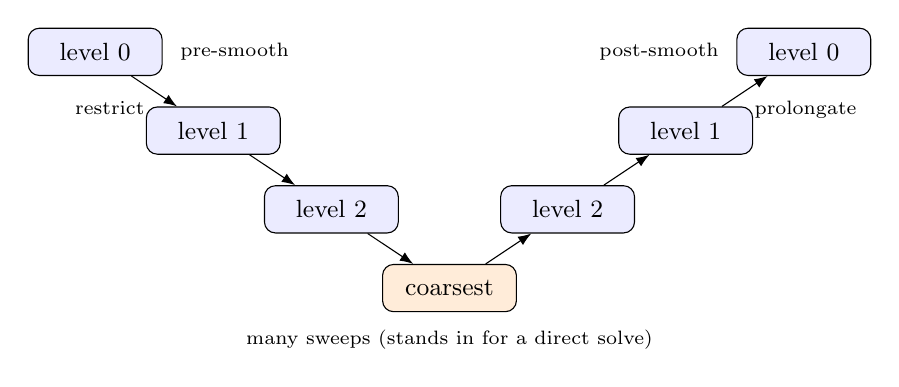
\begin{tikzpicture}[>=Latex, scale=1.0,
  lev/.style={draw, rounded corners, fill=blue!8, minimum width=17mm, minimum height=6mm, font=\small}]
  \node[lev] (f0) at (0,0)      {level 0};
  \node[lev] (f1) at (1.5,-1.0) {level 1};
  \node[lev] (f2) at (3.0,-2.0) {level 2};
  \node[lev, fill=orange!15] (c) at (4.5,-3.0) {coarsest};
  \node[lev] (g2) at (6.0,-2.0) {level 2};
  \node[lev] (g1) at (7.5,-1.0) {level 1};
  \node[lev] (g0) at (9.0,0)    {level 0};
  \draw[->] (f0)--(f1) node[midway,below left,font=\scriptsize]{restrict};
  \draw[->] (f1)--(f2);
  \draw[->] (f2)--(c);
  \draw[->] (c)--(g2);
  \draw[->] (g2)--(g1);
  \draw[->] (g1)--(g0) node[midway,below right,font=\scriptsize]{prolongate};
  \node[font=\scriptsize, align=left, right=1mm of f0] {pre-smooth};
  \node[font=\scriptsize, align=left, left=1mm of g0] {post-smooth};
  \node[font=\scriptsize, below=1mm of c] {many sweeps (stands in for a direct solve)};
\end{tikzpicture}
\caption{One multigrid V-cycle. Pre- and post-smoothing sweeps run on every level that
has a coarser one beneath it.}
\label{fig:vcycle}
\end{figure}

\begin{table}[h]
\centering
\caption{Multigrid configuration (\texttt{ConfigMultigrid}).}
\label{tab:mg}
\begin{tabular}{@{}>{\raggedright\arraybackslash}p{0.26\linewidth}
                   >{\raggedright\arraybackslash}p{0.10\linewidth}
                   >{\raggedright\arraybackslash}p{0.56\linewidth}@{}}
\toprule
\textbf{Setting} & \textbf{Default} & \textbf{Meaning} \\
\midrule
\texttt{maxIter}            & 3   & V-cycles per pressure-correction solve. This is an \emph{inner} solve inside SIMPLE's outer loop, so it does not need to converge---a few cycles is the usual trade. Exposed as \textbf{Maximum Multigrid Cycles}. \\
\texttt{weight}             & 0.6 & Damping on the weighted-Jacobi smoother. The under-relaxation is what makes Jacobi \emph{smooth} the high-frequency error the coarse grid cannot see; at 1.0 it stops being a smoother and the V-cycle stalls. \\
\texttt{linearSweep}        & 30  & Sweeps used as the coarsest-level solve. Exposed as \textbf{Coarsest Level Sweeps}. \\
\texttt{linearPrePostSweep} & 3   & Sweeps before restriction and again after prolongation, on every level that has a coarser one beneath it. \\
\bottomrule
\end{tabular}
\end{table}

The whole V-cycle is captured into a \textbf{CUDA graph} and replayed each iteration
rather than re-launching every kernel individually (Section~\ref{sec:perf}). Because the
graph bakes in the cycle and sweep counts, those two fields are locked once a solve has
prepared the graph; the GUI disables them with an explanatory tooltip while a run is in
progress.

\subsection{Boundary conditions}\label{sec:bc}
Boundary conditions are applied per boundary group. A group first has a physical
\emph{boundary type} (wall, velocity inlet, pressure outlet, symmetry, or far field),
then each active field on that type has a \emph{condition type} (Dirichlet, Neumann,
fully developed, pulsatile, Michaelis--Menten, Hill, or none). The boundary editor only
shows scalar fields when their solves are enabled.

\begin{table}[h]
\centering
\caption{Boundary types and variables exposed by the editor.}
\label{tab:bc}
\begin{tabular}{@{}>{\raggedright\arraybackslash}p{0.22\linewidth}
                   >{\raggedright\arraybackslash}p{0.28\linewidth}
                   >{\raggedright\arraybackslash}p{0.42\linewidth}@{}}
\toprule
\textbf{Boundary type} & \textbf{Variables} & \textbf{Typical/default treatment} \\
\midrule
Wall & \(u_z\), \(u_r\), optional \(T\), optional \(C\)
     & No-slip velocity; scalar Dirichlet/Neumann or concentration kinetics. \\
Velocity inlet & \(u_z\), \(u_r\), optional \(T\), optional \(C\)
     & Prescribed velocity/scalars; pressure defaults to zero-gradient. Fully developed and pulsatile velocity are allowed when the group orientation is compatible. \\
Pressure outlet & \(p\), optional \(T\), optional \(C\)
     & Prescribed pressure; velocity and concentration default to zero-gradient. The face flux now carries the Rhie--Chow pressure term (Section~\ref{sec:rhiechow}). \\
Symmetry & No editable rows in the GUI
     & Effective defaults enforce the expected zero-normal/zero-gradient symmetry behaviour based on boundary orientation. \\
Far field \newline \emph{(new in v1.05)} & \(u_z\), \(u_r\) values only
     & Freestream velocity values are editable, but the mathematical condition is fixed: \(u_z\) and \(u_r\) are always Dirichlet, and pressure and scalars stay at zero gradient. The editor shows the condition type as read-only text rather than a one-choice combo. \\
\bottomrule
\end{tabular}
\end{table}

\begin{table}[h]
\centering
\caption{Condition types used by boundary variables.}
\label{tab:bctypes}
\begin{tabular}{@{}>{\raggedright\arraybackslash}p{0.25\linewidth}
                   >{\raggedright\arraybackslash}p{0.67\linewidth}@{}}
\toprule
\textbf{Condition type} & \textbf{Meaning} \\
\midrule
Dirichlet & Prescribed field value at the boundary. \\
Neumann & Prescribed normal gradient/flux value; zero gives a zero-gradient boundary. \\
Fully developed & Parabolic fully developed inlet profile using the group's total length and the edited peak/reference value. \\
Pulsatile \emph{(new)} & Time-dependent inlet value \(u(t) = U_0\,[\,1 + A\sin(2\pi f t)\,]\), with mean \(U_0\) (or \(V_0\) on a radial inlet), dimensionless amplitude \(A\), and frequency \(f\) in Hz. Phase is preserved across a continued transient run. \\
Michaelis--Menten & Concentration wall consumption with \(V_{\max}\), \(K_m\), optional inhibition \(m,K_2,V_2\), and optional wall-layer resistance. \\
Hill & Concentration wall consumption with \(V_{\max}\), \(K_m\), Hill exponent \(n\), optional inhibition \(m,K_2,V_2\), and optional wall-layer resistance. \\
None & No condition for that variable/group combination. \\
\bottomrule
\end{tabular}
\end{table}

Wall-layer entries are available for concentration and static temperature on wall
groups. Each layer has a transport coefficient \(k\), thickness \(d\), and derived
resistance \(R=d/k\). The solver uploads the total layer resistance
\(R_{\mathrm{tot}}\) and adds it in series with the cell-to-wall diffusion resistance
when evaluating scalar wall fluxes.

\subsection{Steady and transient runs}\label{sec:transient}
The solver runs steady-state or transient. A transient run is configured from the
\textbf{Transient} node of the solver tree:

\begin{itemize}[nosep]
  \item \textbf{Time Discretization} --- \emph{First Order Implicit} (backward Euler) or
        \emph{Second Order Implicit} (BDF2). BDF2 reads two previous time levels; both
        are allocated unconditionally so the scheme can be changed between runs without
        reallocating.
  \item \textbf{Time step \(dt\)} and \textbf{tEnd} --- the step size and the physical
        end time.
  \item \textbf{Save keyframe every \# iterations} --- how often a snapshot is captured
        into the animation (Section~\ref{sec:animation}).
\end{itemize}

Each time step is driven to convergence by the same SIMPLE outer loop used for steady
runs, so the residual plot shows one converging sawtooth per step
(Figure~\ref{fig:transient}). When the run ends, the console reports the number of time
steps taken and the number of animation frames captured.

\begin{figure}[h]
\centering
\screenshot{ui_transient.png}{0.92\linewidth}{transient settings and residuals}
\caption{A transient run. Each sawtooth in the residual plot is one time step being
driven to convergence; the settings panel holds the time scheme, step size, end time,
and keyframe interval.}
\label{fig:transient}
\end{figure}

\subsection{Convergence and residuals}
Convergence is monitored through residuals plotted live with ImPlot. Residuals can be
computed raw or RMS, with $L_1$, $L_2$, or $L_\infty$ norms and optional scaling by $N$,
$\sqrt{N}$, or the matrix diagonal (\texttt{ResidualType}, \texttt{ResidualNormType},
\texttt{ResidualScalingType}). The primary plotted residuals are \(u_z\), \(u_r\),
continuity, and enabled scalar fields.

\begin{figure}[h]
\centering
\screenshot{ui_solver.png}{0.92\linewidth}{solver tab with live residual plot}
\caption{The Solver tab: solver and linear-solver selection, the multigrid toggle,
discretisation options, and the live residual plot.}
\label{fig:solver}
\end{figure}

\subsection{Derived fields}\label{sec:derived}
\notebox{\textbf{New in v1.05-alpha.} Two fields are derived from the converged velocity
rather than solved for, and appear in the Results tab alongside the solved fields.}

\textbf{Velocity magnitude} is simply \(\lvert\mathbf{V}\rvert = \sqrt{u_z^2 + u_r^2}\).

\textbf{Cell Reynolds number} is
\begin{equation}
\mathrm{Re}_{\text{cell}} = \frac{\rho\,\lvert\mathbf{V}\rvert\,h}{\mu},
\qquad h = \sqrt{A_{2D}},
\end{equation}
where \(h\) is the cell's own length scale, taken as the square root of its \(r\)--\(z\)
cross-section---the one measure that means the same thing on a structured quad, a
multi-block quad, and a triangle. This is the Reynolds number the \emph{discretisation}
sees, not the flow's: it says whether a cell is small enough for the chosen convection
scheme, so it is read against the mesh rather than against the physics. Solid and
inactive cells are left at zero.

Both fields are functions of the final velocity, so---like the gradient fields---they
are not captured per time step, and a transient run leaves them at the final state.

\subsection{GPU acceleration and device data}
At solve time the host \texttt{FVMesh} is packed and uploaded to the device as
\texttt{FVMeshDevice}, which stores cells and faces in structure-of-arrays form with
CSR-style face connectivity (\texttt{faceStart}, \texttt{faceIDs}). Per-field boundary
data is uploaded per group (\texttt{BoundarySolverDevice}). Kernels assemble the
coefficient matrices and run the iterative solves; CUDA streams and events coordinate
and time the work, and the multigrid V-cycle is replayed from a captured CUDA graph.

% ======================================================================
\section{Performance}\label{sec:perf}
% ======================================================================
The v1.05-alpha cycle included a profiling pass on a representative structured case,
captured with NVIDIA Nsight Systems. Table~\ref{tab:perf} lists the wall-clock time
after each optimisation, measured rather than derived.

\begin{table}[h]
\centering
\caption{Measured wall-clock solve time after each optimisation, on the same case and
GPU.}
\label{tab:perf}
\begin{tabular}{@{}>{\raggedright\arraybackslash}p{0.66\linewidth} r@{}}
\toprule
\textbf{Optimisation} & \textbf{Runtime} \\
\midrule
\emph{(baseline)}                                                & $\sim$11.9\,s \\
\texttt{createPPCoeff} fix + \texttt{\_\_forceinline\_\_} face helpers & 11.54\,s \\
Fused residual + Jacobi smoother (\texttt{jacobiFused})          & 8.26\,s \\
CUDA graphs over \texttt{MultigridSolver::run()}                 & 6.61\,s \\
\texttt{computeGradient}: 4500 $\rightarrow$ 3000 calls          & 5.99\,s \\
Single-block coarsest-level Jacobi sweep                         & 5.97\,s \\
\midrule
\textbf{Total} & \textbf{11.9 $\rightarrow$ 5.97\,s ($-50\%$)} \\
\bottomrule
\end{tabular}
\end{table}

Two of these are worth calling out because they are structural rather than incremental:

\begin{itemize}[nosep]
  \item \textbf{Cross-translation-unit inlining.} CUDA separable compilation prevents the
        compiler from inlining device functions across translation units, so the small
        per-face geometry helpers were being called through and spilling to local
        memory. Declaring them \texttt{\_\_forceinline\_\_} in a shared header, taking
        their arguments by \texttt{const\&}, removed the spill.
  \item \textbf{CUDA graphs.} A multigrid V-cycle is many small kernel launches, and at
        this problem size launch overhead dominated the actual arithmetic. Capturing the
        cycle once and replaying the graph cut roughly a quarter of the remaining time.
\end{itemize}

\warnbox{These numbers are a single-machine, single-case measurement taken during
development. They describe the relative effect of each change, not a benchmark of the
software.}

% ======================================================================
\section{Post-processing and Results}
% ======================================================================
\subsection{3D results view}
After a solve, press \textbf{Generate Results} to copy the solver fields into the
post-processing views. The Results tab revolves the 2D solution into a 3D model that
you can orbit, pan, and zoom with an arcball camera (Section~\ref{sec:camera}).
Structured results are drawn with instanced cylindrical strips; unstructured results
are revolved from the triangular finite-volume mesh. The active field is coloured by
the active colormap. Filter controls can show values less than, equal to, greater than,
between, or outside selected thresholds.

\begin{figure}[h]
\centering
\screenshot{ui_results.png}{0.92\linewidth}{3D results view with 2D inspector}
\caption{Results view: a revolved field above the 2D cross-section inspector. The
colorbar sits on the inspector itself and reports the field's display unit; the tab bar
selects which field is shown.}
\label{fig:results}
\end{figure}

\subsection{Field tabs and the shown-field set}
The inspector carries a tab bar of fields rather than a single active field. Which
fields appear there is the \emph{shown set}, edited by drag and drop from the
\textbf{Graphics} picker in the Results panel. Adding a field makes its tab current;
removing the active field falls back to the first remaining tab. After each
\textbf{Generate Results}, the set is re-synchronised: stale names are dropped and the
default flow and scalar fields (axial velocity, radial velocity, velocity magnitude,
continuity, pressure, cell Reynolds number, temperature, concentration) are ensured
present for whichever solves were enabled, while any extra tabs you added are preserved.

\subsection{Mirroring about the axis}
\notebox{\textbf{New in v1.05-alpha.} A \textbf{Mirror} toggle in the ribbon reflects the
2D inspector's field across the axis of symmetry, so the half-plane solution is
displayed as the full cross-section it represents.}

\begin{figure}[h]
\centering
\screenshot{ui_mirror.png}{0.92\linewidth}{mirrored inspector view}
\caption{The same solution with mirroring enabled: the \(r>0\) half-plane the solver
actually computes is reflected to show the full cross-section.}
\label{fig:mirror}
\end{figure}

\subsection{Animation playback}\label{sec:animation}
\notebox{\textbf{New in v1.05-alpha.} A transient run captures keyframes into an
animation that can be replayed in the Results tab.}

Each captured frame stores both halves of what the results views need: the per-cell
\texttt{SolutionField} values that the 2D inspector colours real mesh cells from, and
the raster \texttt{Field} values that the 3D scene samples as a texture. Selecting a
frame pushes its data into the live results state, so every view updates together.

The \textbf{Color Range} control chooses how the colorbar is scaled during playback:

\begin{itemize}[nosep]
  \item \textbf{Global (whole run)} --- the colorbar is pinned to each field's minimum
        and maximum \emph{across every frame}, so a colour means the same value in every
        frame and the legend does not jitter as the animation plays. This is the default.
  \item \textbf{Local (per frame)} --- each frame is scaled to its own range, which
        maximises contrast within a frame at the cost of comparability between frames.
\end{itemize}

\subsection{Data picker (3D)}
Clicking the 3D surface returns the field value at that location. The click ray is
intersected with the cylinder (end caps plus outer surface), and the nearest valid
intersection is used. The value is then obtained by bilinear interpolation of the 2D
solution; because the solution is axisymmetric, only the axial and radial directions
are needed. Care is taken near boundaries because field values are stored at cell
centres.

\subsection{2D inspector and per-cell mesh data}
The 2D inspector renders the solution directly over the finite-volume mesh (each cell
coloured by its value, with flat or interpolated shading) using the same
\texttt{ImDrawList}/2D-camera approach as the sketch and mesh views. A value probe shows
the field value under the cursor, and the picked cell's value is echoed in the console.
The mesh-data inspect tool lets you click a cell to read its geometric and quality
data---centroid, area/volume, face count, per-face neighbour, edge length, and
non-orthogonality, plus, where available, per-cell continuity and face mass fluxes.

\subsection{Colorbar and colormaps}
A colorbar accompanies the field views and is drawn on the inspector itself. Colormaps
(Turbo, Parula, HSV, Gray) are stored as 256-entry lookup tables compiled into the
application; the colorbar and field views sample the active colormap and clamp to each
field's min/max. The display panel lets you choose numeric precision and number format
(General, Fixed, Scientific). The colormap can also be changed, printed, or copied from
the console (Section~\ref{sec:console}).

\notebox{\textbf{Changed in v1.05-alpha.} Three colorbar defects were fixed. Non-finite
samples are now skipped when computing a field's range---a single NaN made the whole
range NaN, which flattened the field to one colour. Tick precision is now chosen per
number format (\%g counts significant digits, \%f counts decimals, \%e counts decimals
plus an exponent) and capped at the $\sim$7 significant digits a \texttt{float} can
actually carry, so the extra digits are no longer rounding noise dressed up as
measurement. Tick values are interpolated in double precision instead of accumulated
from a float step, so the bottom tick prints as the true minimum. The inspector's range
pass also now iterates only over cells it will actually draw, instead of stretching the
colorbar past anything visible.}

% ======================================================================
\section{Interactive Features and Camera}\label{sec:camera}
% ======================================================================
\subsection{3D arcball camera}
The 3D view uses an arcball camera built on quaternions (avoiding gimbal lock). Holding
the middle mouse button and dragging rotates the camera along a spherical path about the
target; the rotation axis and angle come from mapping the previous and current cursor
positions $\hat{\mathbf{V}}_a, \hat{\mathbf{V}}_b$ onto a sphere:
\begin{equation}
\text{Axis} = \frac{\hat{\mathbf{V}}_a \times \hat{\mathbf{V}}_b}{\lvert \hat{\mathbf{V}}_a \times \hat{\mathbf{V}}_b\rvert},
\qquad
\theta = \arccos\!\left(\hat{\mathbf{V}}_a \cdot \hat{\mathbf{V}}_b\right).
\end{equation}
Clicking an axis snaps the camera to an axis-aligned view by \texttt{slerp}-interpolating
from the current to a target orientation.

\subsection{2D camera}
The sketch, mesh, and 2D-inspector views share a 2D camera with wheel zoom and
middle-button pan, plus world/screen coordinate conversion used for picking and
overlays.

\subsection{Mouse picking and gestures}
Selection in 3D uses ray casting against object bounding boxes (slab method); each box
has a unique ID so the program can dispatch the correct action on a hit. In 2D, cell and
boundary picking use point-in-triangle and point-to-segment tests in world space. A
mouse gesture belongs to whatever panel it started on: a left press that landed outside
the mesh canvas can no longer turn into a rubber-band box selection when it is dragged
into it.

% ======================================================================
\section{Console}\label{sec:console}
% ======================================================================
The console accepts text commands, keeps a command history, and offers a live
autocomplete dropdown for registered commands, objects, and values. It is primarily a
utility interface for settings, inspection, copying, and project I/O; solver execution is
controlled from the GUI. Table~\ref{tab:consolecmds} lists the current command families.

\begin{table}[h]
\centering
\caption{Console commands in v1.05-alpha.}
\label{tab:consolecmds}
\begin{tabular}{@{}>{\raggedright\arraybackslash}p{0.32\linewidth}
                   >{\raggedright\arraybackslash}p{0.58\linewidth}@{}}
\toprule
\textbf{Command} & \textbf{Purpose} \\
\midrule
\texttt{set colormap <name>} or \texttt{set cmap <name>}
  & Switch the active colormap. Valid names are the built-in colormap names such as \texttt{Turbo}, \texttt{Parula}, \texttt{HSV}, and \texttt{Gray}. \\
\texttt{get gpu memory} or \texttt{get gpu mem}
  & Print free, total, and used GPU memory. \\
\texttt{get colormap} & Print the active colormap name. \\
\texttt{get colormap <name>} & Print all 256 RGB rows for a named colormap. \\
\texttt{copy residual} & Copy the residual plot image to the clipboard. \\
\texttt{copy mesh} & Copy the mesh inspector image to the clipboard. \\
\texttt{copy inspector} & Copy the 2D result inspector image to the clipboard. \\
\texttt{copy colormap [name]} & Copy RGB rows for the active or named colormap to the clipboard. \\
\texttt{save project} & Open a save dialog and write the whole project. \\
\texttt{load project} & Open a load dialog and reload a whole project. \\
\texttt{tutorial} & Toggle the in-application tutorial overlay. \\
\texttt{clear} or \texttt{clr} & Clear the console output. \\
\texttt{help} & Print registered commands and their usage strings. \\
\texttt{ping} & Diagnostic command; prints \texttt{pong!}. \\
\bottomrule
\end{tabular}
\end{table}

% ======================================================================
\section{Data Structures Reference}
% ======================================================================
Table~\ref{tab:structs} summarises the central data structures. The host
representation (\texttt{FVMesh}, Section~\ref{sec:fvdata}) is the source of truth; a
packed structure-of-arrays form is uploaded to the GPU for solving.

\begin{table}[h]
\centering
\caption{Key data structures.}
\label{tab:structs}
\begin{tabular}{@{}>{\raggedright\arraybackslash}p{0.26\linewidth}
                   >{\raggedright\arraybackslash}p{0.66\linewidth}@{}}
\toprule
\textbf{Structure} & \textbf{Purpose} \\
\midrule
\texttt{Project} & Shared project state that owns \texttt{Geometry}, \texttt{Mesh}, \texttt{Solver}, \texttt{Results}, the current tab, project path/name, simple-view flag, and display length scale. \\
\texttt{SketchModel} & Geometry sketch: points, lines, circles, arcs, rectangles, dimensions, active tool, and ID counters. \\
\texttt{GridConfig} & Structured grid: $n_r, n_z, L, R$, face/centre coordinates, grading, \texttt{activeCell}, \texttt{obstacleIndices}, and device pointers. \\
\texttt{MultiBlockMesh} & Multi-block trellis decomposition: conformal blocks plus the per-band axial/radial cell counts that keep block seams matched. \\
\texttt{FluidPropertyConfig} & Fluid and transport properties: density $\rho$, viscosity $\mu$, $c_p$, $k$, diffusivities, and reaction parameters. \\
\texttt{VariableUnits} & Per-quantity display-unit selection; values are stored in base SI and converted only at the UI edge. \\
\texttt{Triangle} & Three vertex indices; one triangle = one unstructured FV cell. \\
\texttt{FVCell / FVFace / FVMesh} & Host finite-volume mesh: cell geometry, face owner/neighbour/normal/area, connectivity. \\
\texttt{FVMeshDevice} & Device (CUDA) mesh in structure-of-arrays form with CSR face connectivity. \\
\texttt{MeshColoring} & Greedy graph colouring of the cell adjacency graph, so Gauss--Seidel can sweep a colour in place on any mesh type. \\
\texttt{ConfigSolver / ConfigSimple} & Solver configuration: linear solver, schemes, transient/$dt$/$t_{\text{end}}$, time scheme, tolerances, corrector passes. \\
\texttt{ConfigMultigrid} & V-cycle configuration: cycles per solve, smoother weight, coarsest-level and pre/post sweep counts. \\
\texttt{VariablesSimple} & Device field arrays for SIMPLE ($u, v, p, p'$, $T$, $C$, gradients, mass flux), the extra $n-1$ time level used by BDF2, and relaxation factors. \\
\texttt{Coefficients} & Per-field linear-system coefficients ($A_E, A_W, A_N, A_S, A_C, b$, residuals). \\
\texttt{BoundaryCondition / BCParams} & Variant-backed per-variable boundary condition: Dirichlet, Neumann, fully developed, pulsatile, Michaelis--Menten, Hill, or none. \\
\texttt{BoundarySegmentGroup} & A named group of boundary segments carrying a boundary type, per-field boundary conditions, sizing, total length, orientation, and scalar wall layers. \\
\texttt{MeshRegionOfInfluence} & Circular or rectangular unstructured-mesh refinement region with target/outside spacing, transition thickness, and an optional boundary-spacing override. \\
\texttt{BoundaryFieldHost / BoundaryFieldDevice} & Host/device boundary arrays by group: condition type, boundary type, values, length, kinetics parameters, inhibition parameters, and total layer resistance. \\
\texttt{SolutionField} & Host result field and metadata used by the Results tab and 2D inspector. \\
\texttt{Results::AnimationFrame} & One instant of a transient run: its time, its per-cell solutions, and its raster fields. \\
\bottomrule
\end{tabular}
\end{table}

% ======================================================================
\section{Save and Load}
% ======================================================================
Project state is saved to and loaded from binary files to keep file size small and
preserve the internal data structures used by the GUI.

\subsection{File types}
\notebox{\textbf{New in v1.05-alpha.} Each kind of file now has its own extension, so a
project, geometry, mesh, and solver file are distinguishable in Explorer and the load
dialog stops offering files of the wrong type. The loaders read raw structs and never
validate what they were handed, so this filtering is a correctness guard, not only a
convenience. \texttt{.bin} remains as a second filter entry in every dialog, because every
save written before this change used it.}

\begin{table}[h]
\centering
\caption{Project file kinds.}
\label{tab:filekinds}
\begin{tabular}{@{}llp{0.52\linewidth}@{}}
\toprule
\textbf{Kind} & \textbf{Extension} & \textbf{Contents} \\
\midrule
Project  & \texttt{.axi}     & Everything below, plus project metadata and results. \\
Geometry & \texttt{.axigeom} & Sketch geometry only; importable and exportable on its own from the File menu. \\
Mesh     & \texttt{.aximesh} & Mesh state only. \\
Solver   & \texttt{.axislv}  & Solver settings only. \\
Legacy   & \texttt{.bin}     & Any of the above written before v1.05-alpha. \\
\bottomrule
\end{tabular}
\end{table}

\subsection{What a project file stores}
A project file currently stores:
\begin{itemize}[nosep]
  \item sketch geometry, including points, lines, circles, arcs, rectangles,
        dimensions, and ID counters;
  \item mesh state, including structured grid dimensions/spacing, multi-block band cell
        counts, active/obstacle cells, unstructured points/triangles, boundary segments,
        boundary groups, boundary-condition settings, wall-layer settings, and regions
        of influence;
  \item solver settings, including active fields, residual plotting settings, linear
        solver and multigrid settings, SIMPLE settings, transient/time-scheme settings,
        convection scheme, and fluid/transport/reaction properties;
  \item \textbf{results}, including the solved fields and, where present, the captured
        transient animation frames;
  \item project metadata, including project name, project path, display length scale,
        and unit selections.
\end{itemize}

\notebox{\textbf{New in v1.05-alpha.} Results are persisted in the project file. Reloading
a project therefore restores its solution without re-running the solver. Only what cannot
be derived is stored: the render-side data (the raster grid, the cylinder template, the
per-field CPU values and GL textures, and each animation frame's raster field) is rebuilt
on load, and the finite-volume mesh is reconstructed from the mesh when the project was
never solved in this session. Because loading can happen before the OpenGL context
exists---a project reopened at launch is read before the window is created---the rebuild
is deferred to the GUI's next frame rather than run inline. Projects that were saved
before the results format settled still load; their results are simply absent.}

Multi-block state is derived from the sketch rather than serialised, and is rebuilt after
a load so a loaded structured project does not revert to the raster grid in the inspector
and the solver.

The application also writes small local startup files. \texttt{project\_settings.bin}
stores the quick-launch project path, while \texttt{openAtLaunchProject.bin} can store
a snapshot of the current project for reopening at launch. These files are application
state, not portable interchange files.

The solver payload has a small file marker and version field, and selected legacy solver
payloads are fallback-loaded. Even with that guard, the binary format is intended for
this application version and may change between alpha releases. For long-term archiving,
keep screenshots, exported plots/tables, and notes alongside the project file.

% ======================================================================
\section{Limitations}\label{sec:limitations}
% ======================================================================
\begin{itemize}[nosep]
  \item \textbf{Not verified or validated.} Results have not been checked against
        analytical solutions, reference solvers, or experiments (Section~\ref{sec:disclaimer}).
  \item \textbf{Alpha software.} Expect bugs, incomplete features, and breaking changes
        between versions; saved files may not be forward/backward compatible.
  \item \textbf{Results predating v1.05-alpha.} The concentration mass-flux and
        pressure-outlet Rhie--Chow corrections change converged solutions, not just
        run time. Earlier results are not comparable with current ones.
  \item \textbf{Physics scope.} Incompressible, axisymmetric (no swirl/3D), laminar
        flow only---no turbulence modelling. Scalar transport (energy, concentration)
        is passive/one-way unless otherwise configured.
  \item \textbf{Solver scope.} SIMPLE is the implemented and GUI-exposed
        pressure--velocity coupling; other schemes (SIMPLER, SIMPLEC, PISO) are not yet
        available.
  \item \textbf{GUI-exposed linear solvers.} Jacobi and red--black Gauss--Seidel are the
        supported user-facing linear solvers, with multigrid available for the
        pressure-correction solve. Other solver code paths in the repository
        (BiCGSTAB, GMRES) exist but are not exposed and should not be treated as
        validated features.
  \item \textbf{GUI-exposed convection schemes.} First-order upwind, central
        differencing, and second-order upwind. A QUICK scheme exists in the enumeration
        but is not offered in the interface.
  \item \textbf{Multigrid scope.} Multigrid accelerates the pressure correction only,
        not the momentum or scalar solves. Its cycle and sweep counts are baked into the
        captured CUDA graph and cannot be changed mid-run.
  \item \textbf{Multi-block scope.} Multi-block decomposition requires axis-aligned
        rectilinear geometry. Circles, arcs, skewed outline edges, open loops, and
        degenerate rectangles fall back to the rasterised single-block grid.
  \item \textbf{Non-orthogonal correction.} Off by default; the deferred cross term can
        destabilise on skewed or near-axis cells, so it is opt-in and limited.
  \item \textbf{Derived fields in transient runs.} Velocity magnitude, cell Reynolds
        number, and the gradient fields are computed from the final state and are not
        captured per time step, so they do not animate.
  \item \textbf{Console scope.} The console adjusts settings, copies/exports views,
        saves/loads projects, and reports information; it does not currently launch the
        main solver from a text command.
  \item \textbf{Presets.} The File \(\rightarrow\) Open \(\rightarrow\) Presets submenu
        is present but currently has no entries wired up.
  \item \textbf{Platform.} Windows x64 only, and it requires a CUDA-capable NVIDIA GPU
        (compute capability $\geq 7.5$); it will not run on AMD/Intel GPUs or CPU-only
        machines. Single-GPU only.
  \item \textbf{CUDA build target.} The checked-in CMake configuration is currently set
        for a local Ampere target (\texttt{sm\_86}). Release builds must broaden the
        CUDA architecture list or include a PTX fallback before distributing to other
        NVIDIA GPUs.
  \item \textbf{Gmsh licensing.} Unstructured meshing depends on Gmsh; redistribution
        must account for Gmsh's licence terms.
  \item \textbf{Scale / memory.} Large meshes are bounded by GPU memory; very large
        cases may not fit or may be slow. A long transient run additionally holds every
        captured animation frame in host memory.
  \item \textbf{Robustness.} Convergence is sensitive to mesh quality, relaxation
        factors, and boundary conditions; poor inputs can diverge.
\end{itemize}

% ======================================================================
\section*{Appendix A: Default Parameters}
\addcontentsline{toc}{section}{Appendix A: Default Parameters}
% ======================================================================
\begin{table}[h]
\centering
\caption{Selected default grid, fluid, and solver parameters (subject to change).}
\begin{tabular}{@{}lll@{}}
\toprule
\textbf{Parameter} & \textbf{Symbol / field} & \textbf{Default} \\
\midrule
Axial cells        & \texttt{nz}  & 100 \\
Radial cells       & \texttt{nr}  & 170 \\
Domain length      & \texttt{L}   & \(0.01\) m \\
Domain radius      & \texttt{R}   & \(0.0017\) m \\
Density            & \texttt{rho} & \(998\) kg\,m\(^{-3}\) (water) \\
Dynamic viscosity  & \texttt{mu}  & \(1.0518\times10^{-3}\) Pa\,s \\
Specific heat      & \texttt{cp}  & \(4180\) J\,kg\(^{-1}\)K\(^{-1}\) \\
Thermal conduct.   & \texttt{k}   & \(0.6\) W\,m\(^{-1}\)K\(^{-1}\) \\
Concentration diff.& \texttt{D}   & \(3.0277\times10^{-9}\) m\(^2\)s\(^{-1}\) \\
Momentum relax.    & ---          & \(0.7\) \\
Pressure relax.    & ---          & \(0.3\) \\
\midrule
SIMPLE inner iterations   & \texttt{ConfigSimple::maxIter}   & 50 \\
Momentum tolerance        & \texttt{momTol}                  & \(10^{-8}\) \\
Pressure-correction tol.  & \texttt{ppTol}                   & \(10^{-5}\) \\
Linear solver             & \texttt{ConfigSolver::type}      & Jacobi \\
Linear inner iterations   & \texttt{ConfigSolver::maxIter}   & 20 \\
Time scheme               & \texttt{timeScheme}              & First order (backward Euler) \\
Time step                 & \texttt{dt}                      & \(0.1\) s \\
End time                  & \texttt{tEnd}                    & \(2.0\) s \\
\midrule
Multigrid cycles          & \texttt{ConfigMultigrid::maxIter} & 3 \\
Smoother weight           & \texttt{weight}                   & 0.6 \\
Coarsest-level sweeps     & \texttt{linearSweep}              & 30 \\
Pre/post sweeps           & \texttt{linearPrePostSweep}       & 3 \\
\bottomrule
\end{tabular}
\end{table}

% ======================================================================
\section*{Appendix B: What Changed in v1.05-alpha}
\addcontentsline{toc}{section}{Appendix B: What Changed in v1.05-alpha}
% ======================================================================
\begin{table}[h]
\centering
\caption{Summary of v1.05-alpha changes, with the section that documents each.}
\begin{tabular}{@{}>{\raggedright\arraybackslash}p{0.30\linewidth}
                   >{\raggedright\arraybackslash}p{0.50\linewidth}
                   >{\raggedright\arraybackslash}p{0.12\linewidth}@{}}
\toprule
\textbf{Area} & \textbf{Change} & \textbf{Section} \\
\midrule
Physics (correction) & Concentration face flux no longer multiplies by density twice & \ref{sec:scalars} \\
Physics (correction) & Rhie--Chow pressure term applied at fixed-pressure boundaries & \ref{sec:rhiechow} \\
Meshing & Multi-block structured meshing by trellis decomposition & \ref{sec:multiblock} \\
Meshing & Region-of-influence boundary-spacing override & \ref{sec:mesh} \\
Meshing & Monotonic boundary group IDs, with migration on load & \ref{sec:mesh} \\
Solver & Geometric multigrid for the pressure correction & \ref{sec:multigrid} \\
Solver & Gauss--Seidel on all mesh types via graph colouring & \ref{sec:linear} \\
Solver & Second-order (BDF2) time discretisation & \ref{sec:transient} \\
Solver & Pulsatile inlet boundary condition & \ref{sec:bc} \\
Solver & Far-field boundary type & \ref{sec:bc} \\
Solver & Velocity magnitude and cell Reynolds number fields & \ref{sec:derived} \\
Performance & CUDA graph replay, fused smoother, forced device inlining ($-50\%$) & \ref{sec:perf} \\
Results & Transient animation playback with global/local colour range & \ref{sec:animation} \\
Results & Mirroring about the axis & --- \\
Results & Colorbar range, precision, and tick-value fixes & --- \\
Interface & Application-wide ribbon; simple view; project-wide units & \ref{sec:ui} \\
Interface & Sketch copy/paste; axis lines no longer snap targets & --- \\
Files & Per-kind extensions (\texttt{.axi}, \texttt{.axigeom}, \texttt{.aximesh}, \texttt{.axislv}) & --- \\
Files & Results persisted in the project file & --- \\
\bottomrule
\end{tabular}
\end{table}

% ======================================================================
\begin{thebibliography}{9}
% ======================================================================
\bibitem{patankar} S.~V.~Patankar, \emph{Numerical Heat Transfer and Fluid Flow}, Hemisphere, 1980.
\bibitem{versteeg} H.~K.~Versteeg and W.~Malalasekera, \emph{An Introduction to Computational Fluid Dynamics: The Finite Volume Method}, 2nd ed., Pearson, 2007.
\bibitem{ferziger} J.~H.~Ferziger and M.~Peri\'c, \emph{Computational Methods for Fluid Dynamics}, 3rd ed., Springer, 2002.
\bibitem{rhiechow} C.~M.~Rhie and W.~L.~Chow, ``Numerical study of the turbulent flow past an airfoil with trailing edge separation,'' \emph{AIAA Journal}, 21(11), 1983.
\bibitem{briggs} W.~L.~Briggs, V.~E.~Henson, and S.~F.~McCormick, \emph{A Multigrid Tutorial}, 2nd ed., SIAM, 2000.
\bibitem{gmsh} C.~Geuzaine and J.-F.~Remacle, ``Gmsh: a three-dimensional finite element mesh generator with built-in pre- and post-processing facilities,'' \emph{Int.\ J.\ Numer.\ Methods Eng.}, 79(11), 2009.
\bibitem{imgui} O.~Cornut, \emph{Dear ImGui}, \url{https://github.com/ocornut/imgui}.
\end{thebibliography}

\end{document}
